%\RequirePackage[l2tabu, orthodox]{nag}
\RequirePackage{currfile}
\documentclass[12pt]{beamer}
\graphicspath{{Imagenes/}{../Imagenes/}}
\usepackage[utf8]{inputenc}
\usepackage[spanish]{babel}
\usepackage{standalone}
\usepackage{color}
\usepackage[binary-units=true]{siunitx}
\usepackage{hyperref}
\hypersetup{
  colorlinks=true,
  linkcolor=blue,          % color of internal links (change box color with linkbordercolor)
  citecolor=green,        % color of links to bibliography
  filecolor=magenta,      % color of file links
  urlcolor=cyan,           % color of external links
  linkbordercolor={0 0 1}
}
\usepackage{xcolor, soul}
\usepackage{etoolbox}
\usepackage{amsmath}
\usepackage{amsthm}
\usepackage{physics}
\usepackage{multicol}
\usepackage{graphicx}
\usepackage{bookmark}
\usepackage{longtable}
\usepackage{graphicx}
\usepackage{tikz}
\usepackage[siunitx, RPvoltages]{circuitikz}
\usetikzlibrary{mindmap}
\usetikzlibrary{arrows, patterns, shapes, decorations.markings, decorations.pathmorphing}
\usetikzlibrary{matrix,positioning}
\tikzstyle{every picture}+=[remember picture,baseline]
\usepackage[autostyle,spanish=mexican]{csquotes}
\usepackage{pifont}
\usepackage[font=footnotesize,textfont=it]{caption}
\usepackage{tabulary}
\usepackage{booktabs}
\usepackage[outdir=./]{epstopdf}
%\usepackage{epstopdf}
\usepackage{media9}
\usepackage{multimedia}
\usepackage{bigints}
%\usepackage{enumitem}
\usepackage[os=win]{menukeys}
\usepackage{pifont}
\usepackage{pbox}
\usepackage{alltt}
\usepackage{verbatim}
\usepackage{colortbl}
\usepackage{tcolorbox}
\usepackage{fancyvrb}
\usepackage[sfdefault]{roboto}  %% Option 'sfdefault' only if the base font of the document is to be sans serif
%\usepackage[T1]{fontenc}
\setcounter{secnumdepth}{3}
\setcounter{tocdepth}{3}
\DeclareGraphicsExtensions{.pdf,.png,.jpg}
\renewcommand {\arraystretch}{1.5}
\definecolor{ao}{rgb}{0.0, 0.5, 0.0}
\definecolor{aquamarine}{rgb}{0.5, 1.0, 0.83}
\definecolor{kellygreen}{rgb}{0.3, 0.73, 0.09}
\definecolor{bisque}{rgb}{1.0, 0.89, 0.77}
\definecolor{amber}{rgb}{1.0, 0.75, 0.0}
\definecolor{armygreen}{rgb}{0.29, 0.33, 0.13}
\definecolor{alizarin}{rgb}{0.82, 0.1, 0.26}
\definecolor{cadetblue}{rgb}{0.37, 0.62, 0.63}
\newcommand*{\TitleParbox}[1]{\parbox[c]{6cm}{\raggedright #1}}%
\newcommand{\python}{\texttt{python}}
\newcommand{\textoazul}[1]{\textcolor{blue}{#1}}
\newcommand{\azulfuerte}[1]{\textcolor{blue}{\textbf{#1}}}
\newcommand{\funcionazul}[1]{\textcolor{blue}{\textbf{\texttt{#1}}}}
%\normalfont
\usepackage{ccfonts}% http://ctan.org/pkg/{ccfonts}
\usepackage[T1]{fontenc}% http://ctan.or/pkg/fontenc
\renewcommand{\rmdefault}{cmr}% cmr = Computer Modern Roman
\usefonttheme[onlymath]{serif}
\linespread{1.3}
\newcounter{saveenumi}
\newcommand{\seti}{\setcounter{saveenumi}{\value{enumi}}}
\newcommand{\conti}{\setcounter{enumi}{\value{saveenumi}}}
\newcommand{\tikzmark}[1]{\tikz[remember picture] \node[coordinate] (#1) {#1};}

\usepackage{scalerel}[2016-12-29]
\def\stretchint#1{\vcenter{\hbox{\stretchto[440]{\displaystyle\int}{#1}}}}
\def\scaleint#1{\vcenter{\hbox{\scaleto[3ex]{\displaystyle\int}{#1}}}}
\def\bs{\mkern-12mu}

\newtheorem{teo}{}[section]
\usepackage{blkarray}

%reduce el tamaño de letra de la etiqueta equations
\makeatletter
\def\maketag@@@#1{\hbox{\m@th\normalfont\small#1}}
\makeatother

%se usa para la x en itemize
\newcommand{\xmark}{\text{\ding{55}}}

%\AtBeginDocument{\setlength{\tymin}{1em}}


\definecolor{myblue}{rgb}{.8, .8, 1}

\usepackage{empheq}

\newlength\mytemplen
\newsavebox\mytempbox

\makeatletter
\newcommand\mybluebox{%
    \@ifnextchar[%]
       {\@mybluebox}%
       {\@mybluebox[0pt]}}

\def\@mybluebox[#1]{%
    \@ifnextchar[%]
       {\@@mybluebox[#1]}%
       {\@@mybluebox[#1][0pt]}}

\def\@@mybluebox[#1][#2]#3{
    \sbox\mytempbox{#3}%
    \mytemplen\ht\mytempbox
    \advance\mytemplen #1\relax
    \ht\mytempbox\mytemplen
    \mytemplen\dp\mytempbox
    \advance\mytemplen #2\relax
    \dp\mytempbox\mytemplen
    \colorbox{myblue}{\hspace{1em}\usebox{\mytempbox}\hspace{1em}}}

\makeatother



%Se usa la plantilla Warsaw modificada con spruce
\mode<presentation>
{
  \usetheme{Warsaw}
  \setbeamertemplate{headline}{}
  \useoutertheme{default}
  %\usecolortheme{beaver}
  \setbeamercovered{invisible}
}
%\AtBeginSection[]
%{
%\begin{frame}<beamer>{Contenido}
%\normalfont\mdseries
%\tableofcontents[currentsection]
%\end{frame}
%}

\setbeamertemplate{section in toc}[sections numbered]
\setbeamertemplate{subsection in toc}[subsections numbered]
\setbeamertemplate{subsection in toc}{\leavevmode\leftskip=3.2em\rlap{\hskip-2em\inserttocsectionnumber.\inserttocsubsectionnumber}\inserttocsubsection\par}
\setbeamercolor{section in toc}{fg=blue}
\setbeamercolor{subsection in toc}{fg=blue}
\setbeamertemplate{navigation symbols}{}
\setbeamercolor{frametitle}{fg=yellow,bg=blue!70!white}
\setbeamercolor{section in head/foot}{bg=gray!30,fg=red}
%\setbeamercolor{section in head}{bg=green,fg=red}
\setbeamercolor{subsection in head/foot}{bg=gray!30,fg=black}
\setbeamercolor{author in head/foot}{bg=gray!30}
\setbeamercolor{date in head/foot}{fg=blue}

%\mode<presentation>
%{
%  \usetheme{Warsaw}
%  \setbeamertemplate{headline}{}
%  %\useoutertheme{infolines}
%  \useoutertheme{default}
%  \setbeamercovered{invisible}
%  % or whatever (possibly just delete it)
%}

\usepackage{courier}
\usepackage{listingsutf8}
\usepackage{listings}
\usepackage{xcolor}
\usepackage{textcomp}
\usepackage{color}
\definecolor{deepblue}{rgb}{0,0,0.5}
\definecolor{brown}{rgb}{0.59, 0.29, 0.0}
\definecolor{OliveGreen}{rgb}{0,0.25,0}
% \usepackage{minted}

\DeclareCaptionFont{white}{\color{white}}
\DeclareCaptionFormat{listing}{\colorbox{gray}{\parbox{0.98\textwidth}{#1#2#3}}}
\captionsetup[lstlisting]{format=listing,labelfont=white,textfont=white}
\renewcommand{\lstlistingname}{Código}


\definecolor{Code}{rgb}{0,0,0}
\definecolor{Keywords}{rgb}{255,0,0}
\definecolor{Strings}{rgb}{255,0,255}
\definecolor{Comments}{rgb}{0,0,255}
\definecolor{Numbers}{rgb}{255,128,0}

\makeatletter

\newif\iffirstchar\firstchartrue
\newif\ifstartedbyadigit
\newif\ifprecededbyequalsign

\newcommand\processletter
{%
  \ifnum\lst@mode=\lst@Pmode%
    \iffirstchar%
        \global\startedbyadigitfalse%
      \fi
      \global\firstcharfalse%
    \fi
}

\newcommand\processdigit
{%
  \ifnum\lst@mode=\lst@Pmode%
      \iffirstchar%
        \global\startedbyadigittrue%
      \fi
      \global\firstcharfalse%
  \fi
}

\lst@AddToHook{OutputOther}%
{%
  \lst@IfLastOtherOneOf{=}
    {\global\precededbyequalsigntrue}
    {}%
}

\lst@AddToHook{Output}%
{%
  \ifprecededbyequalsign%
      \ifstartedbyadigit%
        \def\lst@thestyle{\color{orange}}%
      \fi
    \fi
  \global\firstchartrue%
  \global\startedbyadigitfalse%
  \global\precededbyequalsignfalse%
}

\lstset{ 
language=Python,                % choose the language of the code
basicstyle=\footnotesize\ttfamily,       % the size of the fonts that are used for the code
numbers=left,                   % where to put the line-numbers
numberstyle=\scriptsize,      % the size of the fonts that are used for the line-numbers
stepnumber=1,                   % the step between two line-numbers. If it is 1 each line will be numbered
numbersep=5pt,                  % how far the line-numbers are from the code
backgroundcolor=\color{white},  % choose the background color. You must add \usepackage{color}
showspaces=false,               % show spaces adding particular underscores
showstringspaces=false,         % underline spaces within strings
showtabs=false,                 % show tabs within strings adding particular underscores
frame=single,   		% adds a frame around the code
tabsize=2,  		% sets default tabsize to 2 spaces
captionpos=t,   		% sets the caption-position to bottom
breaklines=true,    	% sets automatic line breaking
breakatwhitespace=false,    % sets if automatic breaks should only happen at whitespace
escapeinside={\#},  % if you want to add a comment within your code
stringstyle =\color{OliveGreen},
%otherkeywords={{as}},             % Add keywords here
keywordstyle = \color{blue},
commentstyle = \color{black},
identifierstyle = \color{black},
literate=%
         {á}{{\'a}}1
         {é}{{\'e}}1
         {í}{{\'i}}1
         {ó}{{\'o}}1
         {ú}{{\'u}}1
%
%keywordstyle=\ttb\color{deepblue}
%fancyvrb = true,
}

\lstdefinestyle{FormattedNumber}{%
    literate={0}{{\textcolor{red}{0}}}{1}%
             {1}{{\textcolor{red}{1}}}{1}%
             {2}{{\textcolor{red}{2}}}{1}%
             {3}{{\textcolor{red}{3}}}{1}%
             {4}{{\textcolor{red}{4}}}{1}%
             {5}{{\textcolor{red}{5}}}{1}%
             {6}{{\textcolor{red}{6}}}{1}%
             {7}{{\textcolor{red}{7}}}{1}%
             {8}{{\textcolor{red}{8}}}{1}%
             {9}{{\textcolor{red}{9}}}{1}%
             {.0}{{\textcolor{red}{.0}}}{2}% Following is to ensure that only periods
             {.1}{{\textcolor{red}{.1}}}{2}% followed by a digit are changed.
             {.2}{{\textcolor{red}{.2}}}{2}%
             {.3}{{\textcolor{red}{.3}}}{2}%
             {.4}{{\textcolor{red}{.4}}}{2}%
             {.5}{{\textcolor{red}{.5}}}{2}%
             {.6}{{\textcolor{red}{.6}}}{2}%
             {.7}{{\textcolor{red}{.7}}}{2}%
             {.8}{{\textcolor{red}{.8}}}{2}%
             {.9}{{\textcolor{red}{.9}}}{2}%
             {\ }{{ }}{1}% handle the space
         ,%
          %mathescape=true
          escapeinside={__}
          }



\makeatletter
\setbeamertemplate{footline}
{
  \leavevmode%
  \hbox{%
  \begin{beamercolorbox}[wd=.333333\paperwidth,ht=2.25ex,dp=1ex,center]{author in head/foot}%
    \usebeamerfont{author in head/foot} \insertsection
  \end{beamercolorbox}}%
  \begin{beamercolorbox}[wd=.333333\paperwidth,ht=2.25ex,dp=1ex,center]{title in head/foot}%
    \usebeamerfont{title in head/foot} \insertsubsection
  \end{beamercolorbox}%
  \begin{beamercolorbox}[wd=.333333\paperwidth,ht=2.25ex,dp=1ex,right]{date in head/foot}%
    \usebeamerfont{date in head/foot} \textcolor{white}{\insertshortdate{}} \hspace*{2em}
    \textcolor{white}{\insertframenumber{} / \inserttotalframenumber}\hspace*{2ex} 
  \end{beamercolorbox}}%
  \vskip0pt%
\makeatother
\title{\large{Tema 1 - Escalas, condición y estabilidad}}
\subtitle{Curso de Física Computacional}
\author[]{M. en C. Gustavo Contreras Mayén}
\date{\today}
\institute{Facultad de Ciencias - UNAM}
\titlegraphic{
\includegraphics[width=2cm]{Imagenes/escudo-facultad-ciencias}\hspace*{4.75cm}~%
   
\includegraphics[width=2cm]{Imagenes/escudo-unam}
}
\begin{document}
\maketitle
\section*{Contenido}
\frame[allowframebreaks]{\tableofcontents[currentsection, hideallsubsections]}
\fontsize{14}{14}\selectfont
\spanishdecimal{.}
\section{Errores e incertidumbres en computación}
\frame{\tableofcontents[currentsection, hideothersubsections]}
\subsection{Consideraciones}
\begin{frame}
\frametitle{Consideraciones}
Para dar inicio a esta parte del Tema, debemos de considerar que aunque seamos cuidadosos o no, los errores y las incertidumbres son una parte inherente de los computación científica.
\end{frame}
\begin{frame}
\frametitle{Consideraciones}
Algunos de esos errores son debidos a nuestra parte como usuarios, pero otros se deben a la computadora.
\\
\bigskip
Los errores computacionales surgen debido a la limitada precisión con la que los equipos almacenan números o porque los algoritmos o modelos pueden fallar.
\end{frame}
\begin{frame}
\frametitle{Consideraciones}
Haremos una revisión sobre los errores e incertidumbres que se pueden presentar en los cálculos computacionales.
\\
\bigskip
\pause
Recuerda que siendo este el tema inicial, lo que veamos aquí, se debe de extender en el manejo de todo nuestro curso de Física Computacional.
\end{frame}
\section{Fuentes de errores}
\frame{\tableofcontents[currentsection, hideothersubsections]}
\subsection{Fuentes de errores - Teoría}
\begin{frame}
\frametitle{Hablando de errores}
Pensemos que tenemos un programa de alta complejidad.
\\
\bigskip
Para entender el por qué los errores deben ser motivo de preocupación, imaginemos un programa con el siguiente flujo lógico
\begin{equation}
\text{Inicio } \rightarrow U_{1} \rightarrow U_{2} \rightarrow \ldots \rightarrow U_{n} \rightarrow \text{ Fin} 
\label{eq:ecuacion_02_01}
\end{equation}
\end{frame}
\begin{frame}
\frametitle{Hablando de errores}
\begin{equation*}
\text{Inicio } \rightarrow U_{1} \rightarrow U_{2} \rightarrow \ldots \rightarrow U_{n} \rightarrow \text{ Fin} 
\end{equation*}
Donde cada unidad $U$ puede ser una declaración de una tarea o un paso.
\\
\bigskip
Si cada unidad tiene probabilidad $p$ de ser correcta, entonces la probabilidad conjunta $P$ de que todo el programa sea correcto es $P = p^{n}$.
\\
\end{frame}
\begin{frame}
\frametitle{Hablando de errores}
Digamos que tenemos un programa de tamaño mediano con $n = 1000$ pasos y que la probabilidad de que cada paso sea correcto es casi uno, $p \simeq 0.9993$.
\\
\bigskip
Esto significa que terminas con $P \simeq \frac{1}{2}$, es decir, la respuesta final es tan probablemente correcta como equivocada.
\end{frame}
\begin{frame}
\frametitle{Hablando de errores}
El problema es que como científicos, queremos un resultado correcto o al menos en el que la incertidumbre sea pequeña y de tamaño conocido.
\end{frame}
\section{Fuentes de errores computacionales}
\frame{\tableofcontents[currentsection, hideothersubsections]}
\subsection{Fuentes de errores generales}
\begin{frame}
\frametitle{Fuentes de errores computacionales}
Existen al menos cuatro fuentes de errores que se pueden presentar en los cálculos computacionales:
\pause
\setbeamercolor{item projected}{bg=blue!70!black,fg=yellow}
\setbeamertemplate{enumerate items}[circle]
\begin{enumerate}[<+->]
\item Un modelo equivocado.
\item Errores aleatorios.
\item Errores por aproximación
\item Errores por redondeo.
\end{enumerate}
\end{frame}
\subsection{Un modelo equivocado}
\begin{frame}
\frametitle{Un modelo equivocado}
Se presentan cuando nuestra propuesta de modelo no es el pertinente, siendo quizá la parte más crítica ya que antes de continuar, debemos de repasar la parte de la física para resolver debidamente nuestro problema
\end{frame}
\begin{frame}
\frametitle{Un modelo equivocado}
También se consideran los errores tipográficos, introducir valores que no corresponden, ejecutar el programa incorrecto, usar el archivo de datos equivocado, etc.
\\
\bigskip
Sugerencia: \pause \textoazul{Si el número de errores comienza a crecer, es momento de ir a casa o tomar un descanso.}
\end{frame}
\subsection{Errores aleatorios}
\begin{frame}
\frametitle{Errores aleatorios}
Se presenta una imprecisión debida por acontecimientos tales como: fluctuaciones en la electrónica, incidencia de rayos cósmicos, o alguien que se tropieza con un enchufe.
\\
\bigskip
Éstos errores pueden ser raros, pero no tenemos ningún control sobre ellos y su probabilidad aumenta conforme transcurre el tiempo.
\end{frame}
\subsection{Errores por aproximación}
\begin{frame}
\frametitle{Errores por aproximación}
La imprecisión surge de la simplificación de las matemáticas para que un problema pueda ser resuelto en la computadora.
\\
\bigskip
Incluyen la sustitución de series infinitas por sumas finitas, intervalos infinitesimales por finitos, y funciones variables por constantes.
\end{frame}
\begin{frame}
\frametitle{Errores por aproximación}
Por ejemplo
\begin{align}
\begin{aligned}
\sin(x) &= \sum_{n = 1}^{\infty} \: \dfrac{(-1)^{n-1} \: x^{2n - 1}}{(2n - 1)!} \hspace{0.5cm} \mbox{(exacta)} \\
&= \simeq \sum_{n = 1}^{N} \: \dfrac{(-1)^{n-1} \: x^{2n - 1}}{(2n - 1)!} \hspace{0.5cm} \mbox{(algoritmo)} \\
& = \sin(x) + \varepsilon(x, N)
\end{aligned}
\label{eq:ecuacion_02_02}
\end{align}
donde $\varepsilon(x,N)$ es el error por la aproximación, en este caso $\varepsilon$ corresponde a los términos desde $N+1$ hasta $\infty$.
\end{frame}
\begin{frame}
\frametitle{Errores por aproximación}
Dado que el error por la aproximación se genera en el algoritmo que usamos para aproximar la matemática, también se le conoce como \underline{error del algoritmo}.
\end{frame}
\begin{frame}
\frametitle{Errores por aproximación}
Para una buena y razonable aproximación, el error debido por la aproximación debería de reducirse cuando el valor de $N$ se incrementa, y debería de anularse en el límite $N \rightarrow \infty$.
\end{frame}
\begin{frame}
\frametitle{Errores por aproximación}
Para el ejemplo (\ref{eq:ecuacion_02_02}), como la escala de $N$ se fija por el valor de $x$, un pequeño error de aproximación requiere que $ N \geqslant x$.
\\
\bigskip
Por lo que si $x$ y $N$ son valores cercanos entre sí, el error de aproximación será grande.
\end{frame}
\subsection{Errores por redondeo}
\begin{frame}
\frametitle{Errores por redondeo}
La imprecisión se genera por el número finito de dígitos utilizados para almacenar números de punto flotante.
\\
\bigskip
Estos \enquote{errores} son análogos a la incertidumbre en la medición de una cantidad física encontrada en un laboratorio de física.
\end{frame}
\begin{frame}
\frametitle{Errores por redondeo}
El error general de redondeo se acumula a medida que el equipo maneja más números, es decir, a medida que aumenta el número de pasos en un cálculo, y puede hacer que algunos algoritmos se vuelvan inestables con un rápido aumento del error.
\end{frame}
\begin{frame}
\frametitle{Errores por redondeo}
En algunos casos, el error por redondeo puede convertirse en el componente principal en la respuesta, lo que lleva a lo que los expertos informáticos llaman \azulfuerte{basura}.
\end{frame}
\begin{frame}
\frametitle{Errores por redondeo}
Por ejemplo, si la computadora mantiene cuatro decimales, entonces almacenará $\frac{1}{3}$ como $0.3333$ y $\frac{2}{3} = 0.6667$, donde el equipo ha \enquote{redondeado} el último dígito en $\dfrac{2}{3}$.
\end{frame}
\begin{frame}
\frametitle{Errores por redondeo}
Por consiguiente, si hacemos en la computadora un cálculo tan simple como $2 \frac{1}{3} - \frac{2}{3}$, produce
\begin{equation}
2 \left( \dfrac{1}{3} \right) - \dfrac{2}{3} = 0.6666 - 0.6667 = -0.0001 \neq 0
\label{eq:ecuacion_02_03}
\end{equation}
\pause
Aunque el resultado es pequeño, no es $0$, y si se repete este tipo millones de veces este cálculo, la respuesta final puede que ni siquiera sea pequeña (\textcolor{red}{la basura genera basura}).
\end{frame}
\section{Modelos para el desastre}
\frame{\tableofcontents[currentsection, hideothersubsections]}
\subsection{Cancelación en la sustracción}
\begin{frame}
\frametitle{Cancelación en la sustracción}
Un cálculo que utiliza números que se almacenan de manera aproximada en la computadora, puede devolver una solución aproximada.
\\
\bigskip
Para demostrar este hecho, consideremos que hay un valor de incertidumbre, sea $x_{c}$ el valor representado en la computadora del valor exacto $x$, tal que:
\begin{equation}
x_{c} \simeq  x( 1 + \varepsilon_{x})
\label{eq:ecuacion_02_05}
\end{equation}
\end{frame}
\begin{frame}
\frametitle{Cancelación en la sustracción}
\begin{equation*}
x_{c} \simeq  x( 1 + \varepsilon_{x})
\end{equation*}
Donde $\epsilon_{x}$ es el error relativo de $x_{c}$, el cual se espera que sea similar en magnitud al épsilon de la máquina $\epsilon_{m}$.
\end{frame}
\begin{frame}
\frametitle{Cancelación en la sustracción}
Si usamos ésta notación para una diferencia entre dos valores $a = b - c$, tenemos que:
\begin{align}
\begin{aligned}
a = b - c & \Rightarrow a_{c} \simeq b_{c} - c_{c} \simeq b(1 + \epsilon_{b}) - c(1 + \epsilon_{c}) \\
{} & \Rightarrow \dfrac{a_{c}}{a} \simeq 1 + \epsilon_{b} \dfrac{b}{a} - \dfrac{c}{a} \epsilon_{c}
\end{aligned}
\label{eq:ecuacion:02_06}
\end{align} 
\end{frame}
\begin{frame}
\frametitle{Cancelación en la sustracción}
Vemos que el error resultante en $a$ es un promedio de los errores en $b$ y $c$, y no hay seguridad en que los dos términos se cancelen.
\end{frame}
\begin{frame}
\frametitle{Cancelación en la sustracción}
El error en $a_{c}$ se incrementa cuando se restan dos valores cercanos $(b \simeq c)$, porque entonces estamos restando las partes más significativas de ambos números y dejando las partes menos significativas propensas a errores:
\begin{equation}
\dfrac{a_{c}}{a} \stackrel{def}{=} 1 + \epsilon_{a} \simeq 1 + \dfrac{b}{a}(\epsilon_{b} - \epsilon_{c}) \simeq 1 + \dfrac{b}{a} \: max(\vert \epsilon_{b} \vert, \vert \epsilon_{c} \vert) 
\label{eq:ecuacion_02_07}
\end{equation}
\end{frame}
\begin{frame}
\frametitle{Cancelación en la sustracción}
Esto muestra que incluso si los errores relativos en $b$ y $c$ pueden cancelar algo, se multiplican por número grande $b / a$, lo que puede aumentar significativamente el error.
\\
\bigskip
Debido a que no podemos asumir ningún signo de los errores, debemos asumir el peor escenario: el máximo en la expresion (\ref{eq:ecuacion_02_07}).
\end{frame}
\subsection{Ejercicio 1}
\begin{frame}
\frametitle{Ejercicio 1}
Aprendimos en la secundaria a resolver la ecuación homogénea de segundo grado:
\begin{equation}
a \: x^{2} + b \: x + c = 0
\label{eq:ecuacion_02_08}
\end{equation}
que tiene una solución analítica que se puede escribir como
\\
\medskip
\begin{align}
\begin{aligned}
x_{1, 2} &= \dfrac{-b \pm \sqrt{b^{2} - 4 \: a \: c}}{2 \: a} \hspace{0.5cm} \mbox{ o } \\
\\
x_{1^{\prime}, 2^{\prime}} &= \dfrac{-2 \: c}{b \pm \sqrt{b^{2} - 4 \: a \: c}}
\end{aligned}
\label{eq:ecuacion_02_09}
\end{align}
\end{frame}
\begin{frame}
Revisando la expresión anterior (\ref{eq:ecuacion_02_09}) vemos que la cancelación en la sustracción aumenta (y por tanto, un incremento en el error) cuando $b^{2} \gg 4 \: a \: c$ debido a que la raíz cuadrada y el siguiente término están muy próximos a cancelarse.
\end{frame}
\begin{frame}
\frametitle{Manos al código}
\setbeamercolor{item projected}{bg=blue!70!black,fg=yellow}
\setbeamertemplate{enumerate items}[circle]
\begin{enumerate}[<+->]
\item Escribe un programa que calcule las cuatro soluciones para valores arbitrarios de $a$, $b$ y $c$. \\
Considera las siguientes expresiones:
\begin{align*}
x^{2} - 5 \: x + 6 = 0 \\
- x^{2} - 7 \: x + 3 = 0 \\
x^{2} + 2 \: x + 2 = 0 \\
x^{2} + 3 \: x + 1 = 0
\end{align*}
\seti
\end{enumerate}
\end{frame}
\begin{frame}
\frametitle{Manos al código}
\setbeamercolor{item projected}{bg=blue!70!black,fg=yellow}
\setbeamertemplate{enumerate items}[circle]
\begin{enumerate}[<+->]
\conti
\item Revisa cómo los errores obtenidos en los cálculos, aumentan conforme hay una cancelación en la sustracción de términos y su relación con la precisión de la máquina. Prueba con los siguientes valores $a=1$, $b=1$, $c=10^{-n}, n = 1, 2, 3, \ldots$
\item Estima el error relativo para los valores obtenidos, considera que la expresión que devuelve $x_{1}, x_{2}$ es la del valor exacto.
\seti
\end{enumerate}
\end{frame}
\begin{frame}
\frametitle{Manos al código}
\setbeamercolor{item projected}{bg=blue!70!black,fg=yellow}
\setbeamertemplate{enumerate items}[circle]
\begin{enumerate}[<+->]
\conti
\item Con los valores de error y de $n$, genera una gráfica. Interpreta lo que obtienes.
\item Cómo mejorarías el programa para obtener la mayor precisión en tu respuesta?
\end{enumerate}
\end{frame}
\subsection{Ejercicio 2}
\begin{frame}
\frametitle{Ejercicio 2: Suma 1}
Del ejercicio anterior, hemos visto que la cancelación en la sustracción de los términos se presentan cuando se suma una serie con signos alternantes.
\\
\bigskip
\pause
Consiera ahora la siguiente suma:
\begin{equation}
S^{(1)}_{N}= \sum^{2 \: N}_{n=1} (-1)^{n} \dfrac{n}{n + 1}
\label{eq:ecuacion_02_10}
\end{equation}
\end{frame}
\begin{frame}
\frametitle{Ejercicio 2: Suma 2}
Si sumamos de manera separada los valores impares y los pares de $x$, tendremos dos sumas:
\begin{equation}
S^{(2)}_{N}= - \sum^{N}_{n = 1} \dfrac{2 \: n-1}{2 \: n} + \sum^{N}_{n = 1} \dfrac{2 \: n}{2 \: n + 1}
\label{eq:ecuacion_02_11}
\end{equation}
En esta expresión, todos los términos son positivos con sólo una sustracción al final del cálculo.
\end{frame}
\begin{frame}
\frametitle{Ejercicio 2: Suma 3}
Podemos eliminar la diferencia mediante una combinación entre las dos sumas anteriores, quedando de la siguiente manera
\begin{equation}
S^{(3)}_{N}=  \sum^{N}_{n = 1} \dfrac{1}{2 \: n \: (2 \: n + 1)}
\label{eq:ecuacion_02_12}
\end{equation}
\end{frame}
\begin{frame}
\frametitle{Revisando las tres sumas}
Sabemos que aunque el valor de las tres sumas $S^{(1)}_{N}$, $S^{(2)}_{N}$, $S^{(3)}_{N}$, es el mismo, el resultado númerico puede ser diferente.
\setbeamertemplate{enumerate items}[circle]
\begin{enumerate}[<+->]
\item Escribe un programa que calcule $S^{(1)}_{N}$, $S^{(2)}_{N}$, $S^{(3)}_{N}$.
\seti
\end{enumerate}
\end{frame}
\begin{frame}
\frametitle{Revisando las tres sumas}
\setbeamercolor{item projected}{bg=blue!70!black,fg=yellow}
\setbeamertemplate{enumerate items}[circle]
\begin{enumerate}[<+->]
\conti
\item Supongamos que $S^{(3)}_{N}$ es el valor exacto de la suma. Grafica el error relativo contra el número de términos en la suma (tip: usa una escala log-log). Comienza con $N = 1$ hasta $N = 1000000$. Describe la gráfica.
\item Identifica en tu gráfica una región en donde la tendencia es casi lineal, ¿qué representa ésta sección con respecto al error?
\end{enumerate}
\end{frame}
\section{Errores por redondeo}
\frame{\tableofcontents[currentsection, hideothersubsections]}
\subsection{Errores por redondeo en un paso}
\begin{frame}
\frametitle{Error por redondeo en un paso}
Comencemos por ver cómo surge el error en una división con las representaciones de computadora de dos números:
\begin{align}
\begin{aligned}
a = \dfrac{b}{c} &\Rightarrow a_{c} = \dfrac{b_{c}}{c_{c}} = \dfrac{b \ (1 + \varepsilon_{b})}{c \: (1 + \varepsilon_{c})} \\
&\Rightarrow \dfrac{a_{c}}{a} = \dfrac{1 + \varepsilon_{b}}{1 + \varepsilon_{c}} \simeq (1 + \varepsilon_{b}) \: (1 - \varepsilon_{c}) \simeq 1 + \varepsilon_{b} - \varepsilon_{c} \\
&\Rightarrow \dfrac{a_{c}}{a} \simeq 1 + \vert \varepsilon_{b} \vert + \vert \varepsilon_{c} \vert
\label{eq:ecuacion_02_13}
\end{aligned}
\end{align}
\end{frame}
\begin{frame}
\frametitle{Error por redondeo en un paso}
Aquí se han ignorado los términos muy pequeños $\varepsilon^{2}$ y se han añadido errores en valor absoluto ya que no podemos asumir que tenemos la suerte de tener errores desconocidos que se cancelan entre sí.
\end{frame}
\begin{frame}
\frametitle{Error por redondeo en un paso}
Debido a que añadimos los errores en valor absoluto, esta misma regla se aplica a la multiplicación.
\\
\bigskip
La ecuación (\ref{eq:ecuacion_02_13}) es sólo la regla básica de la propagación de errores a partir del trabajo que se hace en un laboratorio:
\end{frame}
\begin{frame}
\frametitle{Error por redondeo en un paso}
\textoazul{Se suman las incertidumbres en cada cantidad involucrada en un análisis para llegar a la incertidumbre general.}
\end{frame}
\subsection{Errores por redondeo en varios pasos}
\begin{frame}
\frametitle{Errores por redondeo en varios pasos}
Existe un modelo útil para aproximar cómo se acumula el error de redondeo en un cálculo que implica un gran número de pasos.
\end{frame}
\begin{frame}
\frametitle{Errores por redondeo en varios pasos}
Consideremos el error en cada paso como un \enquote{paso} literal en una \emph{caminata aleatoria\footnote{Parte del contenido del Tema de Métodos de Montecarlo}}, es decir, una caminata para la cual cada paso está en una dirección aleatoria.
\end{frame}
\begin{frame}
\frametitle{Errores por redondeo en varios pasos}
La distancia total recorrida en $N$ pasos de longitud $r$, es en promedio:
\begin{equation}
R \simeq \sqrt{N} \: r
\label{eq:ecuacion_02_17}
\end{equation}
\pause
Por analogía, el error relativo total $\varepsilon_{0}$ que se genera luego de $N$ pasos computacionales cada uno, con un error de precisión de la máquina $\varepsilon_{m}$, es en promedio
\begin{equation}
\varepsilon_{ro} \simeq \sqrt{N} \: \varepsilon_{m}
\label{eq:ecuacion_02_18}
\end{equation}
\end{frame}
\begin{frame}
\frametitle{Errores por redondeo en varios pasos}
Si los errores de redondeo en un algoritmo particular no se acumulan de manera aleatoria, entonces \textoazul{se necesita un análisis detallado para predecir la dependencia del error en el número de pasos $N$}.
\\
\bigskip
En algunos casos no puede haber cancelación, y el error puede aumentar como $N \: \varepsilon_{m}$.
\end{frame}
\begin{frame}
\frametitle{Conclusión sobre los errores por redondeo}
Nuestra discusión de los errores tiene una implicación importante que hay que tener presente antes de ser impresionado por un cálculo que requiere horas de ejecución.
\\
\bigskip
\pause
Un equipo rápido puede completar $10^{10}$ operaciones de punto flotante por segundo.
\end{frame}
\begin{frame}
\frametitle{Conclusión sobre los errores por redondeo}
Esto significa que un programa que se ejecuta durante $3$ horas realiza aproximadamente $10^{14}$ operaciones.
\\
\bigskip
Por lo tanto, si el error de redondeo se acumula aleatoriamente, después de $3$ horas esperamos un error relativo de $10^{7} \: \varepsilon_{m}$.
\end{frame}
\begin{frame}
\frametitle{Conclusión sobre los errores por redondeo}
Para que el error sea menor que la respuesta, necesitamos que $\varepsilon_{m} < 10^{-7}$, lo que requiere doble precisión y un buen algoritmo.
\\
\bigskip
Si queremos una respuesta de mayor precisión, \emph{\textoazul{entonces necesitaremos un algoritmo muy bueno.}}
\end{frame}
\section{Errores en las funciones esféricas de Bessel}
\frame[allowframebreaks]{\tableofcontents[currentsection, hideothersubsections]}
\subsection{Funciones de Bessel}
\begin{frame}
\frametitle{Funciones de Bessel}
La acumulación de errores por redondeo a menudo limita la capacidad de un programa para calcular con precisión.
\\
\bigskip
\pause
Revisaremos como ejercicio, la manera de calcular las funciones esféricas de Bessel $j_{\ell}(x)$ y de Neumann $n_{\ell}(x)$.
\end{frame}
\begin{frame}
\frametitle{Funciones de Bessel}
Estas funciones son respectivamente, las soluciones regulares/irregulares (no singulares / singulares en el origen) de la ecuación diferencial
\begin{equation}
x^{2} \: f^{\prime \prime} (x) + 2 \: x \: f^{\prime}(x) + [ x^{2} - \ell ( \ell + 1)] \: f(x) = 0
\label{eq:ecuacion_02_19}
\end{equation}
\end{frame}
\begin{frame}
\frametitle{Funciones de Bessel y esféricas de Bessel}
Las funciones esféricas de Bessel se relacionan con las funciones de Bessel de primera clase por
\[ j_{\ell}(x) = \sqrt{\dfrac{\pi}{2 \: x}} \: J_{n + \frac{1}{2}} (x) \]
\end{frame}
\begin{frame}
\frametitle{Funciones de Bessel y esféricas de Bessel}
Se encuentran en diversos problemas de la física, coo la expansión de una onda plana en ondas esféricas parciales
\begin{equation}
e^{i \: \mathbf{k \cdot r}} = \sum_{\ell = 0}^{\infty} i^{\ell} \: (2 \: \ell + 1) \: j_{\ell} (k \:  r) \: P_{\ell}(\cos \theta)
\label{eq:ecuacion_02_20}
\end{equation}    
\end{frame}
\begin{frame}
\frametitle{Funciones esféricas de Bessel de orden $n$}
\fontsize{12}{12}\selectfont
A continuación se muestra una gráfica con las funciones esféricas de Bessel de orden $n = 0, \ldots, 5$:
\begin{figure}
\centering
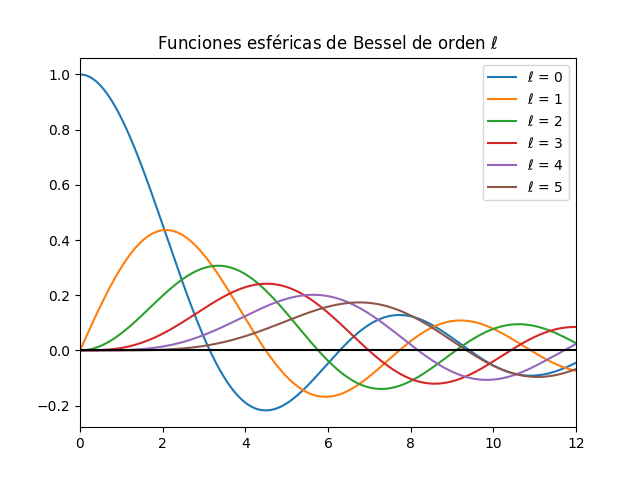
\includegraphics[scale=0.4]{funcionesEsfericasBessel}
\caption{La gráfica se generó usando la librería de funciones especiales de \python.}
%\caption{Nótese que para valores pequeños de $x$, los valores para un $\ell$ mayor, se hacen prograsivamente más pequeños.}
\end{figure}
\end{frame}
\begin{frame}
\frametitle{Valores para $\ell = 0, 1$}
Los dos primero valores para $\ell$ son
\begin{align}
j_{0} (x) &= + \dfrac{\sin x}{x}, \hspace{1cm} j_{1} (x) = +\dfrac{\sin x}{x^{2}} - \dfrac{\cos x}{x} \label{eq:ecuacion_02_21} \\
&{} \nonumber \\
n_{0} (x) &= - \dfrac{\cos x}{x}, \hspace{1cm} n_{1} (x) = -\dfrac{\cos x}{x^{2}} - \dfrac{\sin x}{x} \label{eq:ecuacion_02_22}
\end{align}
\end{frame}
\subsection{Ejercicio: Relaciones de recursión}
\begin{frame}
\frametitle{Relaciones de recursión}
La manera clásica de calcular las funciones de Bessel de orden $j$: $j_{\ell} (x)$ es sumar su serie de potencias para valores pequeños de $\frac{x}{\ell}$ y sumando su expansión asintótica para valores de $x$ grandes.
\end{frame}
\begin{frame}
\frametitle{Relaciones de recurrencia}
El enfoque que usaremos, se basa en \emph{las relaciones de recurrencia}:
\begin{align}
j_{\ell + 1} (x) = \dfrac{2 \: \ell + 1}{x} \: j_{\ell}(x) - j_{\ell - 1}(x) \hspace{0.5cm} \mbox{hacia arriba} \label{eq:ecuacion_02_23}  \\
{} \nonumber \\ 
j_{\ell - 1} (x) = \dfrac{2 \: \ell + 1}{x} \: j_{\ell}(x) - j_{\ell + 1}(x) \hspace{0.5cm} \mbox{hacia abajo} \label{eq:ecuacion_02_24}
\end{align}
\end{frame}
\begin{frame}
\frametitle{Relaciones de recurrencia}
Las ecuaciones (\ref{eq:ecuacion_02_23}) y (\ref{eq:ecuacion_02_24}) son la misma relación:
\setbeamercolor{item projected}{bg=blue!70!black,fg=yellow}
\setbeamertemplate{enumerate items}[circle]
\begin{enumerate}[<+->]
\item Una escrita para la recurrencia hacia adelante que parte de valores pequeños a valores grandes de $\ell$.
\item La otra relación de recurrencia es descendente para valores de $\ell$ pequeños.
\end{enumerate}
\pause
 Con unas cuantas sumas y multiplicaciones, las relaciones de recurrencia permiten el cálculo rápido y sencillo de todo el conjunto de valores de $j_{\ell}$ para $x$ fijo y todo $\ell$.
\end{frame}
\begin{frame}
\frametitle{Relaciones de recurrencia}
Para la relación de recurrencia hacia adelante de $\ell$ para un $x$ fijo, comenzamos con las formas conocidas para $j_{0}$ y $j_{1}$ (\ref{eq:ecuacion_02_21}) y usamos (\ref{eq:ecuacion_02_23}).
\end{frame}
\begin{frame}
\frametitle{Relaciones de recurrencia}
Como veremos, esta recurrencia hacia adelante parece funcionar al principio, pero luego falla.
\\
\bigskip
La razón de la falla se puede ver en las gráficas de $j_{\ell}(x)$ y $n_{\ell}(x)$ como función de $x$.
\end{frame}
\begin{frame}
\frametitle{Relaciones de recurrencia}
\begin{figure}
\centering
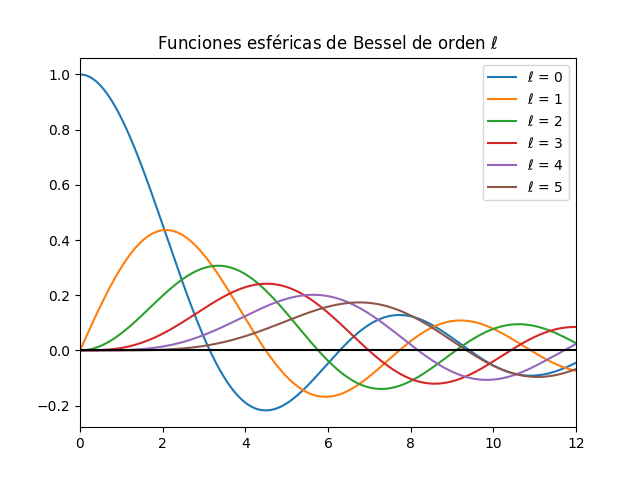
\includegraphics[scale=0.5]{funcionesEsfericasBessel}
\end{figure}
\end{frame}
\begin{frame}
\frametitle{Relaciones de recurrencia}
 Si iniciamos con  $x \simeq 2$ y $\ell = 0$, veremos que a medida que con la  recurrencia hacia adelante para  $j_{\ell}$ con valores mayores de $\ell$ con (\ref{eq:ecuacion_02_23}), esencialmente tomamos la diferencia de dos funciones \enquote{grandes} para producir un valor \enquote{pequeño} para $j_{\ell}$.
\end{frame}
\begin{frame}
\frametitle{Relaciones de recurrencia}
Este proceso sufre de cancelación sustractiva y siempre reduce la precisión.
\\
\bigskip
A medida que continuamos con la recurrencia, tomamos la diferencia de dos funciones pequeñas con errores grandes y producimos una función más pequeña con un error aún mayor. Después de cierto tiempo, nos quedamos con sólo el error de redondeo (basura).
\end{frame}
\begin{frame}
\frametitle{Estimando el error}
Para ser más específicos, llamemos $j_{\ell}^{(c)}$ al valor numérico que calculamos como nua aproximación para $j_{\ell}(x)$.
\\
\bigskip
Por lo que si comenzamos con un valor neto $j_{\ell}$, después de un corto tiempo la falta de precisión de la computadora se mezcla efectivamente en un poco de $n_{\ell}$:
\begin{equation}
j_{\ell}^{(c)} = j_{\ell} (x) + \varepsilon \: n_{\ell} (x)
\label{eq:ecuacion_02_25}	
\end{equation}
\end{frame}
\begin{frame}
\frametitle{Estimando el error}
Esto no lo podemos evitar, porque tanto $j_{\ell}$ como $n_{\ell}$ satisfacen la misma ecuación diferencial y, por esa razón, la misma relación de recurrencia.
\\
\bigskip
La mezcla de $n_{\ell}$ se convierte en un problema cuando el valor numérico de $n_{\ell}(x)$ es mucho mayor que el de $j_{\ell} (x)$ porque incluso una cantidad minúscula de un número muy grande puede ser grande.
\end{frame}
\begin{frame}
\frametitle{Estimando el error}
Por el contrario, si usamos la relación de recurrencia hacia adelante (\ref{eq:ecuacion_02_23}) para generar la función esférica de Neumann $n_{\ell}$, no habrá ningún problema porque estamos combinando funciones pequeñas para producir más grandes, ya que es un proceso que no contiene cancelación sustractiva.
\end{frame}
\begin{frame}
\frametitle{Solución al problema}
La solución simple a este problema es usar (\ref{eq:ecuacion_02_24}) para la recursión descendente de los valores de $j_{\ell}$ que comienzan en un valor grande $\ell = L$.
\\
\bigskip
Esto evita la cancelación sustractiva tomando valores pequeños de $j_{\ell + 1} (x)$ y $j_{\ell}(x)$ y generando por la suma un valor mayor en $j_{\ell -1}(x)$.
\end{frame}
\begin{frame}
\frametitle{Solución al problema}
Mientras que el error todavía puede mantenerse como una función de Neumann, la magnitud real del error disminuirá rápidamente conforme la recurrencia hacia atrás use valores pequeños de $\ell$.
\end{frame}
\begin{frame}
\frametitle{Solución al problema}
De hecho, si empezamos iterando hacia atrás con valores arbitrarios para $j_{L + 1}^{(x)}$ y $j_{L}^{(c)}$, después de un corto tiempo llegaremos a la correcta relación de $\ell$ para este valor de $x$.
\end{frame}
\begin{frame}
\frametitle{Solución al problema}
Aunque el valor numérico de $j_{0}^{c}$ así obtenido no será correcto porque depende de los valores arbitrarios asumidos para $j_{L + 1}$ y $j_{L}^{(c)}$, los valores relativos serán precisos. 
\end{frame}
\begin{frame}
\frametitle{Solución al problema}
Los valores absolutos se fijan a partir del valor conocido (\ref{eq:ecuacion_02_21}), $j_{0} (x) = \sin x / x$.
\\
\bigskip
Debido a que la relación de recurrencia es una relación lineal entre los valores de $j_{\ell}$, sólo necesitamos normalizar todos los valores calculados mediante 
\end{frame}
\begin{frame}
\frametitle{Solución al problema}
\begin{equation}
j_{\ell}^{\text{normalizada}} = j_{\ell}^{(c)} (x) \times \dfrac{j_{0}^{\text{analitica}}}{j_{0}^{(c)}}
\label{eq:ecuacion_02_26}
\end{equation}
En consecuencia, después de haber terminado la recurrencia hacia abajo, se obtendrá la respuesta final normalizando todos los valores de $j_{\ell}^{(c)}$ basados en el valor conocido para $j_{0}$.
\end{frame}
\begin{frame}[fragile]
\frametitle{Propuesta de código}
Veamos la manera de implementar un código con \python para calcular el valor de la función esférica de Bessel con la recurrencia hacia atrás.
\end{frame}
\begin{frame}[allowframebreaks, fragile]
\frametitle{Propuesta de código}
\begin{lstlisting}[style= FormattedNumber, basicstyle=\linespread{0.9}\ttfamily\small, columns=fullflexible]
import numpy as np
import matplotlib.pyplot as plt
import scipy.special as spl

Xmax = 40.
Xmin = 0.25
paso = 0.1
orden = 10; inicio = 50

def abajo (x, n, m):
     j = np.zeros( (inicio + 2), float)
     j[m+1] = j[m] = 1.
     
     for k in range(m, 0, -1):
         j[k-1] = ((2.*k+1.)/x)*j[k] - j[k+1]
     
     escala = (np.sin(x)/x)/j[0]
     
     return j[n] * escala

valores_y = []
valores_x = []

for x in np.arange(Xmin, Xmax, paso):
    valores_y.append(abajo(x, orden, inicio))
    valores_x.append(x)

plt.plot(valores_x, valores_y, color='r')
plt.axhline(y=0, ls='dashed', color = 'k')
plt.xlim([0.25, 40])
plt.show()
\end{lstlisting}
\end{frame}
\begin{frame}
\frametitle{Función aproximada}
\begin{figure}
\centering
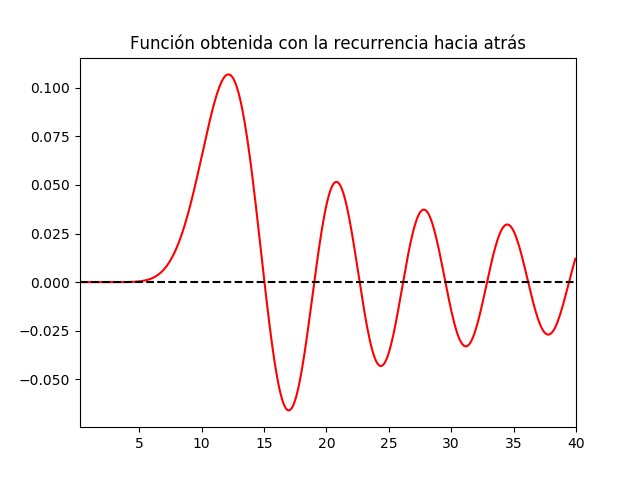
\includegraphics[scale=0.5]{funcionesEsfericasBessel_02}
\caption{Gráfica obtenida con el algoritmo propuesto}
\end{figure}
\end{frame}
\end{document}